%%%%%%%%%%%%%%%%%%%%%%%%%%%%%%%%%%%%%%%%%%%%%%%%%%%%%%%%%%%%%%%%%%%%%%%%%%%%%%%%
%2345678901234567890123456789012345678901234567890123456789012345678901234567890
%        1         2         3         4         5         6         7         8
% THESIS CHAPTER


\chapter{Control Framework}
\label{chap:control}
\ifpdf
    \graphicspath{{ControlFramework/Figures/PNG/}{ControlFramework/Figures/PDF/}{ControlFramework/Figures/}}
\else
    \graphicspath{{ControlFramework/Figures/EPS/}{ControlFramework/Figures/}}
\fi

\section*{Introduction}
In this section, the control framework implemented is discussed. The architecture is constituted by two parts:
\begin{itemize}
	\item The Mission Manager, which job is to supervision the execution of the overall mission. It provides the \textit{action}, a list of control objective that the Kinematic Control Layer must satisfy.
	\item The Kinematic Control Layer (KCL) focus on provide the system velocities (i.e. vehicle and joint velocities), given the list of control objectives from the Mission Manager.
\end{itemize}

This architecture is build from the ones used in \cite{IntroMaris2}, \cite{tesiWander}, \cite{IntroRecent}. The sections \ref{sec:definitions}, \ref{sec:controlObjectives}, \ref{sec:tpik}, \ref{sec:armVehScheme}, and \ref{sec:coopScheme} derive from these works and are here recalled.

\section{Definitions}
\label{sec:definitions}
In this section, principal used notations are described.
\begin{itemize}
	\item The system configuration vector of the robot $ \boldsymbol{c} \in \mathbb{R}^{n}$, ~
	$\boldsymbol{c} \triangleq 
		\begin{bmatrix}
			{\boldsymbol{q}} \\ \boldsymbol{\eta}
		\end{bmatrix}$,\\
	where $\boldsymbol{q} \in \mathbb{R}^{l}$ is the l-DOF arm configuration vector and  $\boldsymbol{\eta} \in \mathbb{R}^6$ is the vehicle \emph{generalized coordinate position vector}. The first three components of $\boldsymbol{\eta}$ are the position vector $\boldsymbol{\eta}_1 \triangleq \begin{bmatrix}x \\ y \\ z\end{bmatrix}$, with components in the inertial frame $\langle w \rangle$. The last three components of $\eta$ are the orientation vector $\boldsymbol{\eta}_2 \triangleq \begin{bmatrix}\phi \\ \theta \\ \psi\end{bmatrix}$ expressed in terms of the three angles roll, pitch, yaw (applied in the yaw-pitch-roll sequence \cite{fossenAnglesSeq}). The singularity given by this Euler sequence that arise when $ \theta = \pi/2$ is handled by a specific control objective (i.e. \textit{horizontal attitude}).
	(TODO) %todo linka sez) 
	From the explained definition, it results that $ n = l+6 $
	
	\item The system velocity vector or the robot $\dot{\boldsymbol{y}} \in \mathbb{R}^n$, ~
	$\dot{\boldsymbol{y}} \triangleq 
	\begin{bmatrix}\dot{\boldsymbol{q}} \\ \boldsymbol{v}\end{bmatrix}$,\\
	where $\dot{\boldsymbol{q}} \in \mathbb{R}^{l}$ are the arm joint velocities and $\boldsymbol{v} \in \mathbb{R}^{6}$ is the vehicle velocity vector. The first three component of $\boldsymbol{v}$ are the linear velocities $\boldsymbol{v}_1 \triangleq \begin{bmatrix}\dot{x} \\ \dot{y} \\ \dot{z}\end{bmatrix}$ and the last three are the angular velocities $\boldsymbol{v}_2 \triangleq \begin{bmatrix}p \\ q \\ r\end{bmatrix}$, both with components in the vehicle frame $\langle v \rangle$. The vehicle is considered fully actuated, so the vector $\dot{\boldsymbol{y}}$ concincides with the control vector used by the kinematic layer.
\end{itemize}
	
\section{Control Objectives}
\label{sec:controlObjectives}
Let us consider what the robot need to achieve. An \textit{objective} is a job that the robot must accomplish during the mission. Different objectives can be requested at the same time, for example we want the joints to stay away from their physical limits, the robot to maintain an horizontal attitude, and the end-effector to reach a desired pose.
\subsection{Control Objectives classification}
\label{sec:coClass}
Control objectives can be classified in order of importance in the execution of the mission. Some of them can be more important of others. For example, usually we prefer that the robot do not hurt humans over the reaching of a goal. Another example could be that the robot should first act to not damage itself while accomplish the mission. In general this give the idea that the more important objectives have to been satisfied first, and then, \textit{if possible}, also the less important ones. 
A general classification based on the \textit{priority} is given here (from the more important class to the less important one):
\begin{itemize}
	\item \textit{Physical Constraints} objectives. This include interaction with environment (e.g not push against a rigid surface, impose a cooperative tool velocity).
	\item \textit{System Safety} objectives, e.g. avoiding joint limits or obstacles.
	\item \textit{Prerequisite} objectives. This is for objectives needed to accomplish the mission, like focus the camera on the object to be grasped
	\item \textit{Mission} objectives, the actual objective that define the mission, like reach an end-effector position.
	\item \textit{Optimization} objectives, to choose, among the possible solution (if multiple ones exist) the best one. To example, to choose the one which has the best energy efficiency.  
\end{itemize}

\subsection{Equality and Inequality Objectives}
We consider a variable  $ \boldsymbol{x}(\boldsymbol{c}) \in \mathbb{R}^m $, dependent on the robot configuration vector $ \boldsymbol{c}$, with $ p $ the control objective \textit{dimension}. The control objective can be of two types:
\begin{itemize}
	\item \textit{Equality control objective}, the requirement, for $t \to \infty$, that \\ \mbox{$\boldsymbol{x}(\boldsymbol{c}) = \boldsymbol{x}_0$}.
	
	\item \textit{Inequality control objective}, the requirement, for $t \to \infty$, that \\ \mbox{$\boldsymbol{x}(\boldsymbol{c}) < \boldsymbol{x}_{max}$ ~ or ~ $\boldsymbol{x}(\boldsymbol{c}) > \boldsymbol{x}_{min}$ ~or ~$ \boldsymbol{x}_{min} < \boldsymbol{x}(\boldsymbol{c}) < \boldsymbol{x}_{max}$}.
\end{itemize}
Please note that here symbols $= , < , >$ refers to element-by-element comparison of the vectors.\\

\subsection{Reactive and non Reactive Control Task}
\label{sec:reactNonReact}
For each control objective, there is always an associated \textit{feedback reference rate}. The aim is to drive the variable $\boldsymbol{x}(\boldsymbol{c})$ toward a point $ \boldsymbol{x}^* $ where the control objective requisite is satisfied. The used example of \textit{feedback reference rate} is:
\begin{equation}
	\boldsymbol{\dot{{\bar{x}}}} (\boldsymbol{x}) \triangleq \gamma (\boldsymbol{x}^* - \boldsymbol{x}),\quad \gamma > 0
\end{equation}
That is a simple proportional law, where $\gamma$ is a positive gain proportional to the desired convergence rate for the considered variable.\\

To link the considered variable $ \boldsymbol{x}(\boldsymbol{c})$ to the system velocity vector, the following relationship is used:
\begin{equation}
\label{eq:CartJacVel}
	\dot{\boldsymbol{x}} = \boldsymbol{J} \dot{\boldsymbol{y}}
\end{equation} 
that express how system velocity vector $\dot{\boldsymbol{y}}$ influences the rate of change of the variable. $ \boldsymbol{J} \in \mathbb{R}^{m \times n}$ is the so-called \textit{task-induced Jacobian}.\\
Having the actual $\dot{\boldsymbol{x}}$ as much as possible equal to the desired reference $\boldsymbol{\bar{x}}$ is called \textit{reactive control task}.\\

There are situation where a task has not an associated control objective. For example, it happens when an external command (e.g. an human operator, or an imposed vehicle velocity) provide directly the reference velocities. In this case, there is no desired $\boldsymbol{x}^*$ to reach, and the reference is generated by something else. It this case, we speak about \textit{non-reactive control task}.

%As an example, we take the objective is to drive the end-effector in a desired pose, with only the arm and considering a fixed vehicle. This problem is well know as \textit{inverse kinematic} problem; i.e. finding the joint velocities $\dot{\boldsymbol{q}} \in \mathbb{R}^l$ which bring the pose $\boldsymbol{x} \in \mathbb{R}^6$ in a specific one. In this case we have:
%\begin{equation}
%\dot{\boldsymbol{x}} = \begin{bmatrix}
%	\underset{3\times3}{\boldsymbol{J_{k,0}}} & \underset{3\times3}{\boldsymbol{0}} \\  \underset{3\times3}{\boldsymbol{0}} & \underset{3\times3}{^{w}\boldsymbol{R}_v}
%	\end{bmatrix}	
%	\dot{\boldsymbol{q}}	
%\end{equation}

%todo ACTIONS? se le uso...

\subsection{Control Objectives Activation and Deactivation}
\label{sec:activations}
During the execution of a mission, not always each inequality control control objective is relevant. As an example, maintaining joints away from their mechanical limits is a safety task which is needed only when the joints are actually near its limits. When a joint is sufficiently far away, there is no necessity to overconstrain the system imposing a velocity. To deal with this, we speak about \textit{activation} and \textit{deactivation} of control objectives and their relative control task.
Let us define the following \textit{activation function}:
\begin{equation}
	a(x) \in [0,1]
\end{equation}
as a continuous, sigmoidal, function, which assumes $0$ value outside the validity region of the control objective, and $1$ inside it. In between, a smooth transition is present, to gently activate/deactivate the control objective. \\
For example, considering a scalar ($ p = 1 $) inequality control objective with the requirement $x(\boldsymbol{c}) > x_{min}$ the \textit{activation function} is defined as:
\begin{equation}
	\label{eq_activation_f}
	a(x) \triangleq
	\begin{cases}1,& x(\boldsymbol{c}) < x_{min}\\
	s(x),& x_{min} \leq x(\boldsymbol{c}) \leq x_{min} + \Delta\\
	0, & x(\boldsymbol{c}) > x_{min} + \Delta\\
	\end{cases}
\end{equation}    
where $s(x)$ is a smooth decreasing function joining the two extreme value $1$ and $0$, and $\Delta$ a value to create a zone where the inequality is satisfied but the activation is between $1$ and $0$ to prevent chattering problems. Similar definition can be done for the other two kind of inequality control objectives.\\

In general, when multidimensional control objectives ($m > 1$) are present, the activation takes the form of a diagonal matrix:
\begin{equation}
\boldsymbol{A} \triangleq
	\begin{bmatrix}
	a_1 & & \\
	& \ddots & \\
	& & a_m	 
	\end{bmatrix}
\end{equation}

Obviously, for equality control tasks the activation is not defined, because they are always \enquote{active}.\\
For \textit{non-reactive} control tasks, the activation is simply $\boldsymbol{A} \equiv 	\begin{bmatrix}
1 & & \\
& \ddots & \\
& & 1	 
\end{bmatrix}$, being absent the variable $x(\boldsymbol{c})$


\section{Task Priority Inverse Kinematics}
\label{sec:tpik}
We describe an \textit{Action} $\mathcal{A}$ as list of prioritized control objectives. Each objectives is positioned at a defined priority level $k$. With this notation, the following symbols are defined:
\begin{itemize}
	\item $\dot{\bar{\boldsymbol{x}}}_k \triangleq \begin{bmatrix}\dot{\bar{x}}_{1,k} & \cdots & \dot{\bar{x}}_{k_m,k}\end{bmatrix}^T$ is the vector of the reference velocities for the control task $k$, of dimension $k_m$.
	\item $\dot{\boldsymbol{x}}_k \triangleq \begin{bmatrix}\dot{x}_{1,k} & \cdots & \dot{x}_{k_m,k}\end{bmatrix}^T$ is the current rate of change of the $k$ task.
	\item $\boldsymbol{J}_k$ is the Jacobian relationship which relates the current rate-of-change $\dot{\boldsymbol{x}}_k$ with the system velocity vector $\dot{\boldsymbol{y}}$ as in equation \eqref{eq:CartJacVel}.
	\item $\boldsymbol{A}_k \triangleq \textrm{diag}(a_{1,k},  \cdots,  a_{k_m,k})$ is the diagonal matrix of all the activation functions described in section \ref{sec:activations}
\end{itemize}
It is important to notice that different objectives can have same priorities $k$. In this case, it is possible to simply stack the vectors and matrices to obtain a objective and a related task $k$ that includes both objectives. Without loss of generality, different objectives will be considered always at different priority levels.

The aim of the kinematic layer is to find the system velocity vector $\boldsymbol{\bar{y}}$ that satisfies \textit{as much as possible} the requirements of each objective of the action $\mathcal{A}$. Given the presence of different objectives with different priorities, it must be taken into account to satisfy higher priority objective first. To do this, a sequence of nested minimization problems must be solved: 
\begin{equation}\label{eq:rminproblem}
S_k \triangleq \left\{ \arg \mathrm{R\textrm{-}}\min_{\dot{\bar{\boldsymbol{y}}} \in S_{k-1}} \left\| \boldsymbol{A}_k (\dot{\bar{\boldsymbol{x}}}_k - \boldsymbol{J}_k \dot{\bar{\boldsymbol{y}}}) \right\|^2 \right\},\, k = 1, 2, \ldots, N,
\end{equation}
where $S_0 \triangleq \mathbb{R}^n$, $S_{k-1}$ is the manifold of solutions of all the previous tasks in the hierarchy, and $N$ is the total number of priority levels. This is the so called \textit{Task Priority Inverse Kinematic} (TPIK). The notation $\mathrm{R\textrm{-}}\min$ is introduced in \cite{IntroMaris1}. The so called \textit{iCAT} (inequality Constraints And Task transitions) framework solve the \eqref{eq:rminproblem} with the algorithm \ref{alg:icat}.\\
\begin{algorithm}[H]
	\caption{iCAT} \label{alg:icat}
	\begin{algorithmic} [1] {\large
		\STATE{$\boldsymbol{\rho}_{0} = \boldsymbol{0}$}
		\STATE{$\boldsymbol{Q}_{0} = \boldsymbol{I}$}
		\vspace{5px}
		\FOR{k=1 \TO N}
		\vspace{5px}
		\STATE{$\boldsymbol{W}_k =  \boldsymbol{J}_k \boldsymbol{Q}_{k-1} (\boldsymbol{J}_k \boldsymbol{Q}_{k-1})^{\#,\boldsymbol{A}_k,\boldsymbol{Q}_{k-1}}$}
				\vspace{5px}
		\STATE{$\boldsymbol{Q}_k = \boldsymbol{Q}_{k-1} (\boldsymbol{I} - (\boldsymbol{J}_k \boldsymbol{Q}_{k-1})^{\#,\boldsymbol{A}_k,\boldsymbol{I}} {\boldsymbol{J}_k \boldsymbol{Q}_{k-1}})$}
		\vspace{5px}
		\STATE{$\boldsymbol{\rho}_k = \boldsymbol{\rho}_{k-1} + \textrm{Sat}\left( \boldsymbol{Q}_{k-1} (\boldsymbol{J}_k \boldsymbol{Q}_{k-1})^{\#,\boldsymbol{A}_k,\boldsymbol{I}} \boldsymbol{W}_k \left(\dot{\bar{\boldsymbol{x}}}_k - \boldsymbol{J}_k \boldsymbol{\rho}_{k-1} \right) \right)$}
		\vspace{5px}
		\ENDFOR 
		\vspace{5px}
		\STATE{$\dot{\boldsymbol{\bar{y}}} = \boldsymbol{\rho}_N$}}
	\end{algorithmic}
\end{algorithm}

\noindent The special pseudo inverse operator $\boldsymbol{(\cdot)}^{\#,\boldsymbol{A},\boldsymbol{Q}}$ [\cite{IntroMaris1}] manages some invariance problems of \eqref{eq:rminproblem}; the function Sat($\cdot$) [\cite{antoSat}] controls the variable saturations. Details of the procedure can be found again in [\cite{IntroMaris1}].

\subsection{Notes on Conflicting Objectives}
From section \ref{sec:coClass}, it should be understood that lower priority task are not always satisfied. The problem with this arise when the main mission objective, that is not at the higher priority, can't be never accomplished, thus failing the general mission. This can be the case with an obstacle: the robot may stuck in a point of \textit{local minima} (that is anyway better than crash into it). This is a general problem of all reactive controlling method. The solution must be found at the mission manager level, which should plan another path or another sequence of Actions. This problem is not considered in this work. 

%todo
%%\subsection{Notes on underactuation} %todo ? vedi un po


\section{Arm-Vehicle Coordination Scheme}
\label{sec:armVehScheme}
\begin{figure}[H]
	\begin{center}
		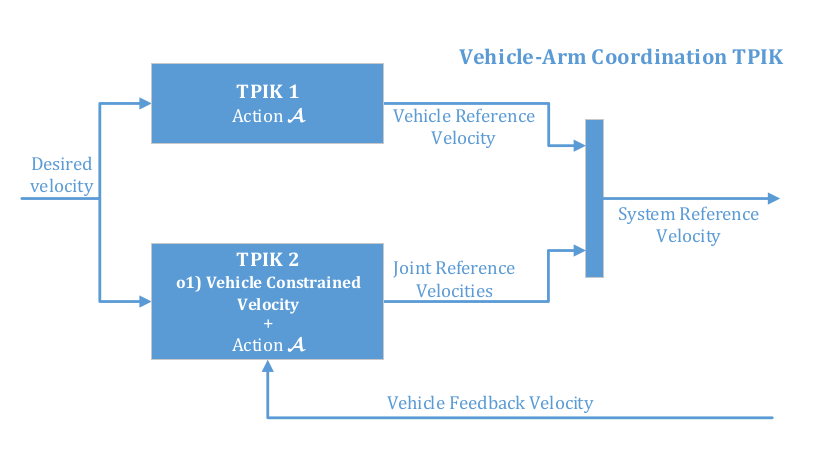
\includegraphics[width=0.90\columnwidth]{vehArmCoordScheme}
		\caption[Arm-Vehicle Coordination Scheme in the TPIK]{A scheme showing the two Task Priority Inverse Kinematics blocks for the arm-vehicle coordination implementation}\label{fig:veharmcoord}
	\end{center}
\end{figure}
Inaccuracy in velocity tracking for vehicle can have effects on the arm. 
A relevant problem arises when disturbances of the floating base, caused by thrusters or its large inertia, propagate and affect the end effector motions [\cite{IntroMaris2}].
To solve this, a kinematic decoupling of arm and base is done, implementing it within the task priority approach The idea is to have two parallel TPIK as shown in \ref{fig:veharmcoord}:
\begin{itemize}
	\item The first TPIK 1, given the Action $\mathcal{A}$ consider the vehicle together with the arm as a whole full controllable system. From its output $\dot{\boldsymbol{\bar{y}}}$ only the vehicle reference velocity are taken.
	\item The second TPIK 2 consider the vehicle as totally non controllable. So, a \textit{non-reactive} task (\ref{sec:reactNonReact})  is used at the top of the priority list to \textit{constrain} the output velocities of the vehicles to the actual one. From the total output $\dot{\boldsymbol{\bar{y}}}$, only the manipulator part is taken.\\
	In this way, the manipulator velocity are \textit{optimized} to follow \textit{at best} the objectives of the action $\mathcal{A}$ considering the \textit{measured} vehicle velocity and their influence on the objectives.	
\end{itemize}

In general, a multi-rate control of arm and vehicle is used, which means that velocities for arm and vehicle are given at different frequency. This schema is suitable for such an implementation: the TPIK 2 can run at higher frequency, updating the manipulator commanded velocities more frequently that the vehicle commanded ones.

\section{Cooperation Scheme}
\label{sec:coopScheme}
\begin{figure}[H]
	\begin{center}
		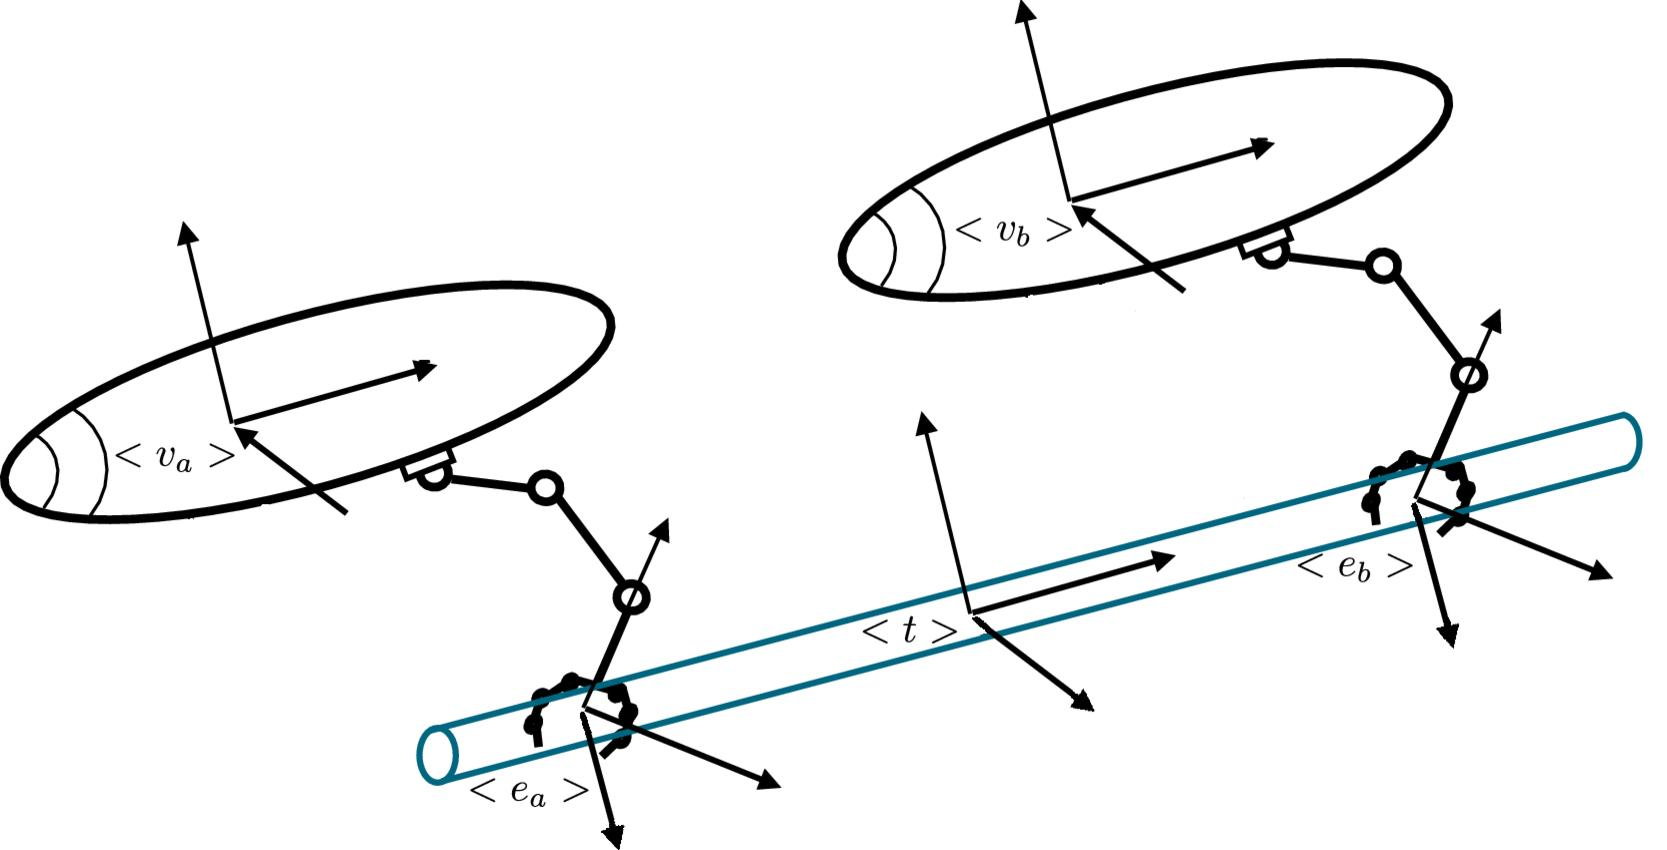
\includegraphics[width=0.60\columnwidth]{coopFrames.jpg}
		\caption{The frames of the two cooperative vehicles carrying a common object}\label{fig:coopFrames}
	\end{center}
\end{figure}

The discussion about cooperation is here explained, limiting it to include only two cooperating robotic systems. This is used to transporting a common object. The coordination policy described take care of the bandwidth restriction in underwater scenario. Thus, it deals with the cooperation in a decentralized manner, limiting the exchange of information.\\
It is assumed that the object is held firmly by both agents, so no sliding happens during the missions. The two robots agree on a shared fixed frame, so, their respective tool frames $\langle t_a \rangle$ and $\langle t_b \rangle$ and the object frame $\langle o \rangle$ are coincident: 
\begin{equation*} 
\langle t \rangle \triangleq \langle t_a \rangle = \langle t_b \rangle = \langle o \rangle
\end{equation*}
In the figure \ref{fig:coopFrames}) the cited frames are shown.
The firm grasp assumption imposes that
\begin{equation}\label{eq:coopintro}
	\dot{\boldsymbol{x}}_t = \boldsymbol{J}_{t,a} \dot{\boldsymbol{y}}_a = \boldsymbol{J}_{t,b} \dot{\boldsymbol{y}}_b
\end{equation}
with $\dot{\boldsymbol{x}}_t$ the object velocity with component on $\langle t \rangle$, $\dot{\boldsymbol{y}}_a$ and $\dot{\boldsymbol{y}}_b$ the system velocity vectors of agents $a$ and $b$ as described in section \ref{sec:definitions}, and $\boldsymbol{J}_{t,a}$ the system Jacobians of agents $a$ and $b$ with respect to $\langle t \rangle$. These Jacobians tells how the tool velocities $\dot{\boldsymbol{x}}_t$ are affected by system velocities $\dot{\boldsymbol{y}}_a$ and $\dot{\boldsymbol{y}}_b$. Due to the firm grasp assumptions, the tool velocities generates by $\dot{\boldsymbol{y}}_a$ and $\dot{\boldsymbol{y}}_b$ must be equal.\\

%Let us rewrite the equation \eqref{eq:coopintro} as:
%\begin{equation}\label{eq:coopintro2}
%\begin{gathered}
%\begin{bmatrix}
%\boldsymbol{J}_{t,a} & -\boldsymbol{J}_{t,b}
%\end{bmatrix}
%\begin{bmatrix}
%\dot{\boldsymbol{y}}_a \\ \dot{\boldsymbol{y}}_b
%\end{bmatrix}
%\triangleq \boldsymbol{G}\dot{\boldsymbol{y}}_{ab}=0 \quad \Longleftrightarrow \quad \dot{\boldsymbol{y}}_{ab} \in ker(\boldsymbol{G}),
%\end{gathered}
%\end{equation}
%This represents the subspace where $\dot{\boldsymbol{y}}_{ab}$ is constrained to lay for the firm grasp assumption.\\

The equation \eqref{eq:coopintro} derived from the grasp constrain can be expressed in the Cartesian space as:
\begin{equation}
	\dot{\boldsymbol{x}}_t = \boldsymbol{J}_{t,a} \boldsymbol{J}^\#_{t,a} \dot{\boldsymbol{x}}_t =  \boldsymbol{J}_{t,b} \boldsymbol{J}^\#_{t,b} 
	\dot{\boldsymbol{x}}_t 
\end{equation}
\begin{equation}
\label{eq:constrainMatrixC}
	(\boldsymbol{J}_{t,a} \boldsymbol{J}^\#_{t,a} - \boldsymbol{J}_{t,b} \boldsymbol{J}^\#_{t,b}) 
	\dot{\boldsymbol{x}}_t \triangleq \boldsymbol{C} \dot{\boldsymbol{x}}_t = \boldsymbol{0}
\end{equation}
\begin{equation}
	\dot{\boldsymbol{x}}_t \in ker(\boldsymbol{C}) = Span(\boldsymbol{I} - \boldsymbol{C}^\#\boldsymbol{C})
\end{equation}
The kernel of $\boldsymbol{C}$, called \textit{Cartesian Constraint Matrix}, express the space of achievable object velocities at the current configuration.\\
The idea of the scheme is to put a non-reactive task at the top of the priority, to constrain the desired object velocity $\dot{\boldsymbol{\tilde{x}}}$ in this subspace. In this way both agents can follow this desired object velocity despite the different situation caused by other objectives.\\
\begin{figure}[H]
	\begin{center}
		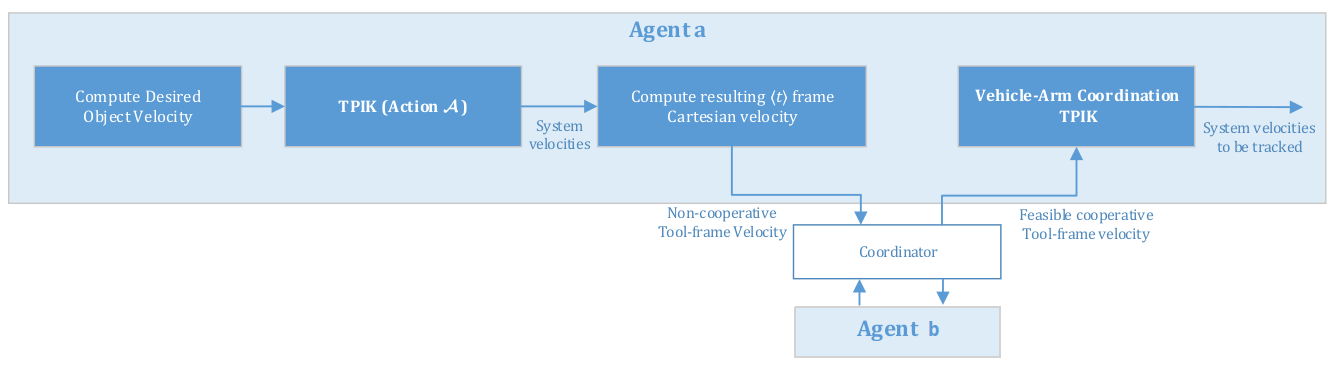
\includegraphics[width=1\columnwidth]{coopScheme.png}
		\caption{The cooperation algorithm with its different steps }\label{fig:coopScheme}
	\end{center}
\end{figure}
The algorithm, schematized in fig. \ref{fig:coopScheme} proceeds as follows:
\begin{itemize}
	\item In the first step, the two agents run the algorithm of \ref{sec:tpik} as they were the only to act. So, we have:
	\begin{equation}
		\dot{\boldsymbol{x}}_{t,a} = \boldsymbol{J}_{t,a} \dot{\boldsymbol{y}}_{a} , \qquad 
		\dot{\boldsymbol{x}}_{t,b} = \boldsymbol{J}_{t,a} \dot{\boldsymbol{y}}_{b}	
	\end{equation}
	where, in general, the two \textit{non cooperative} tool velocities are different: $\dot{\boldsymbol{x}}_{t,a} \neq \dot{\boldsymbol{x}}_{t,b}$.
	
	\item The tool velocities are exchanged (i.e. sent to the coordinator) and a \textit{cooperative} tool velocity is computed:
	\begin{equation}\label{eq:weightsum}
		\dot{\hat{\boldsymbol{x}}}_t = \dfrac{1}{\mu_a + \mu_b} (\mu_a \dot{\boldsymbol{x}}_{t,a}  + \mu_b \dot{\boldsymbol{x}}_{t,b}), \qquad
		\mu_a , \mu_b > 0	
	\end{equation}
    \begin{equation}
		\begin{gathered}
			\mu_a = \mu_0 + \| \dot{\bar{\boldsymbol{x}}}_t - \dot{\boldsymbol{x}}_{t,a} \| \triangleq \mu_0 + \| \boldsymbol{e}_a \|, \\
			\mu_b = \mu_0 + \| \dot{\bar{\boldsymbol{x}}}_t - \dot{\boldsymbol{x}}_{t,b} \| \triangleq \mu_0 + \| \boldsymbol{e}_b \|, \\
			\mu_0 > 0
	    \end{gathered}
	\end{equation}
	where $\dot{\boldsymbol{\bar{x}}}_t$ is the ideal velocity that, if applied, would asymptotically take the tool to the desired goal.\\
	The \textit{cooperative} tool velocity is a \textit{weighted} compromise between the two \textit{non cooperative} ones. The \textit{weights} $\mu_a, \mu_b$ given more freedom to the robot which meet the highest error $\boldsymbol{e}$. This error is a way to understand how much one robot is in difficult in tracking the \textit{ideal} tool velocity $\dot{\boldsymbol{\bar{x}}}_t$.
	
	\item The new \textit{cooperative} tool velocity $\dot{\hat{\boldsymbol{x}}}_t$ is not, in general, a \textit{feasible} velocity that both vehicle can perform. So, an additional passage is required:
	\begin{equation}
		\dot{\tilde{\boldsymbol{x}}}_t \triangleq \big( \boldsymbol{I} - \boldsymbol{C}^\# \boldsymbol{C} \big) \dot{\hat{\boldsymbol{x}}}_t
	\end{equation}
	with $\boldsymbol{C}$ defined in \eqref{eq:constrainMatrixC}.
	
	\item Each agent run a new TPIK procedure, identical to the first one, but with a \textit{non-reactive} control objectives to track the \textit{feasible cooperative} velocity $\dot{\tilde{\boldsymbol{x}}}_t$. The output of the two agents algorithm, $\dot{\boldsymbol{\hat{y}}}_a$ and $\dot{\boldsymbol{\hat{y}}}_b$ will be the final velocity which the kinematic layer provide.\\
	Moving the equality control objective to make the end effector reach the goal at the top of the hierarchy does not influence the safety tasks. This property is proven in \cite{tesiWander}.
\end{itemize}

In this described method, the only information that the agent must exchange are the
\textit{non-cooperative} velocities $\dot{\boldsymbol{x}}_{t,a}, \dot{\boldsymbol{x}}_{t,b}$, the feasible ones $\dot{\boldsymbol{\tilde{x}}}$, and the constrain matrix $\boldsymbol{C}$. Furthermore, even less data can be exchanged if the \textit{coordinator} is a procedure which runs on a robot, and it is not on an external node. 





